% !TEX root = ../document.tex

\chapter{现阶段发展及应用情况}

\section{DLR 的 AOS 实验项目}

\subsection{项目概述}

根据\ref{sec:space_based_ads-b_experiment_back}节的内容,我们得知 DLR 的 AOS(ADS-B over Satellite)项目是世界上第一个天基 ADS-B 可行性验证实验项目。AOS 开发了一个 ADS-B 载荷,作为一个在轨演示器,搭载在 ESA(欧洲航天局)的 PROBA-Vegetation 卫星上,于 2013 年 5 月 7 日被发射到近地轨道上。AOS 是 DLR 空间系统研究所和 DLR 飞行指导研究所的合作项目,与卢森堡合作伙伴 SES TechCom Services 合作。

\renewcommand\arraystretch{1.5}
\begin{table}[htbp]
\centering
\caption{DLR 的 AOS 项目基本描述}
\label{tab:}
\begin{tabular}[b]{|p{2.5cm}<{\raggedleft}|p{12cm}<{\raggedright}|}
\hline
\textbf{目标} & 证明星基 ADS-B 监视的可行性 \par
            搭载于 ESA 的 Proba-V 卫星上的在轨演示器将验证一些关键参数,例如目标截获率、检测率和验证概率 \\
\hline
\textbf{项目持续时间} & 2011 年第一季度至 2014 年第二季度末 \\
\hline
\textbf{合作方} & Institute of Space Systems (RY) in Bremen, Germany \par
        Institute for Flight Guidance (FL) in Braunschweig, Germany \\
\hline
\textbf{贡献} & Institute RY: 开发和组装符合空间要求的 ADS-B 接收机和天线\par
Flight Calibration Services: 开发 ADS-B 接收机\par
Institute FL: ADS-B 数据的验证与评估 \\
\hline
\textbf{更多的合作} & RY with SES-ASTRA / ESA: 提供数据服务器 \\
\hline
\end{tabular}
\end{table}

\renewcommand\arraystretch{1.5}
\begin{table}[htbp]
\centering
\caption{ESA 的 Proba-V 小卫星任务描述}
\label{tab:esa_Proba-V_mission}
\begin{tabular}[b]{|p{2.5cm}<{\raggedleft}|p{12cm}<{\raggedright}|}
\hline
\textbf{主承包商} & QinetiQ Space nv \\
\hline
\textbf{卫星质量} & 约 140kg\\
\hline
\textbf{运载火箭 }& Vega 火箭\\
\hline
\textbf{发射日期} & 2013 年 5 月 7 日 \\
\hline
\textbf{发射场} & 法属圭亚那航天中心(库鲁)\\
\hline
\textbf{发射提供商} & Arianespace \\
\hline
\textbf{轨道} & 太阳同步轨道,海拔 820 公里,倾角 98.73$^\circ$,飘移限制在 10:30AM 到 11:30AM  \\
\hline
\textbf{通信} & 卫星的控制与通信通过比利时 Redu 地面站 \\
\hline
\textbf{主要任务} & 植被扫描仪 \\
\hline
\textbf{载荷} & ADS-B、高能粒子传感器、氮化镓 X 波段功率放大器 \\
\hline
\end{tabular}
\end{table}

ESA Proba-V 卫星自 2013 年 5 月 7 日起进入地球轨道, 其有效载荷包括一个专用接收器,用于接收飞机 ADS-B 信号。5 月 23 日,该实验首次开启,在两小时内在 820 公里的高度记录了 12000 条 ADS-B 信息。飞越苏格兰的 A320 飞机是 DLR 新型接收机从太空“看到”的第一架飞机,证明可以从太空跟踪飞机。


\subsection{体系结构}

Proba-V 上的 ADS-B 接收器由卢森堡的 DLR 和 SES TechCom 提供,主要目的是在飞行代表性配置中测试(空间限定)ADS-B 电路板以评估 TID(总电离剂量)。

ADS-B 接收器(1090ES RX)的基本设计概念是单转换超外差接收机,由 1090MHz 下变频调至中频 70MHz,70MHz 下的 IF 采样由一个 105Msps(每秒兆采样次数)的 16 位 ADC 完成。该 ADS-B 单转换超外差接收机概念如图\ref{fig:dlr_ads-b_receiver}所示\upcite{e2}。

\begin{figure}[htbp]
\centering
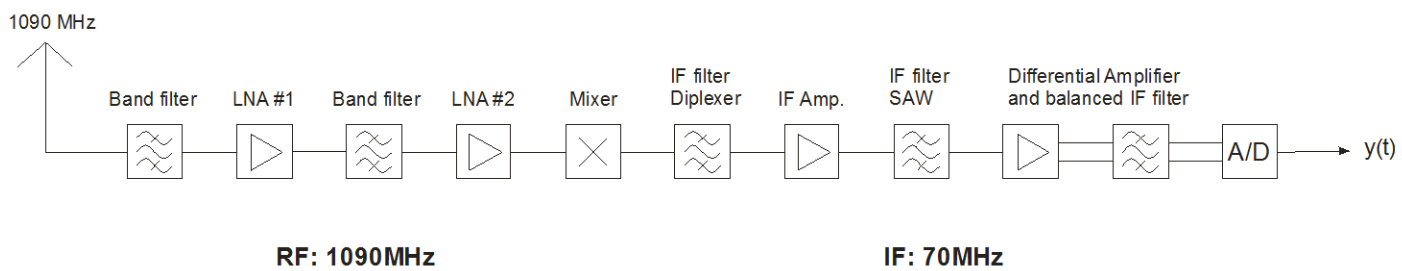
\includegraphics[width=15cm]{pic/dlr_ads-b_receiver.png}
\caption{单转换超外差接收机}
\label{fig:dlr_ads-b_receiver}
\end{figure}

\begin{figure}[htbp]
\centering
\subfigure[载荷原型]{
\begin{minipage}[b]{0.3\linewidth}
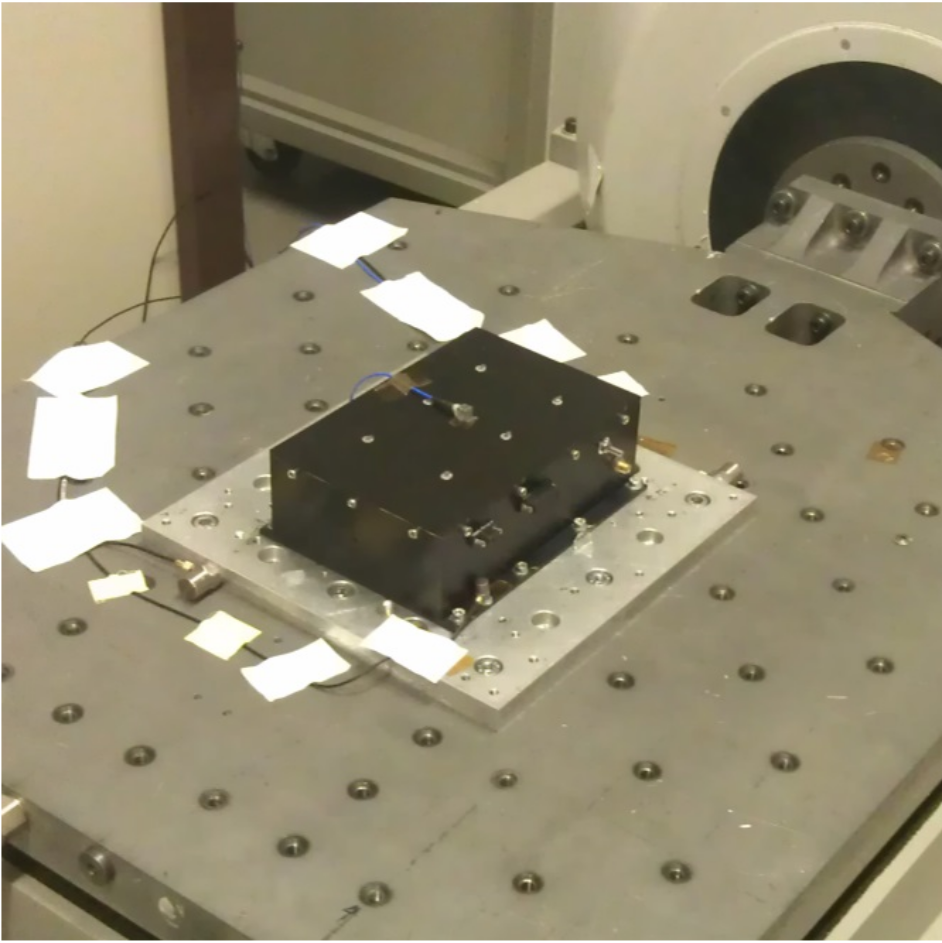
\includegraphics[width=1\linewidth]{pic/aos_ads-b_payload_2.png}
\end{minipage}}
\subfigure[安装位置]{
\begin{minipage}[b]{0.3\linewidth}
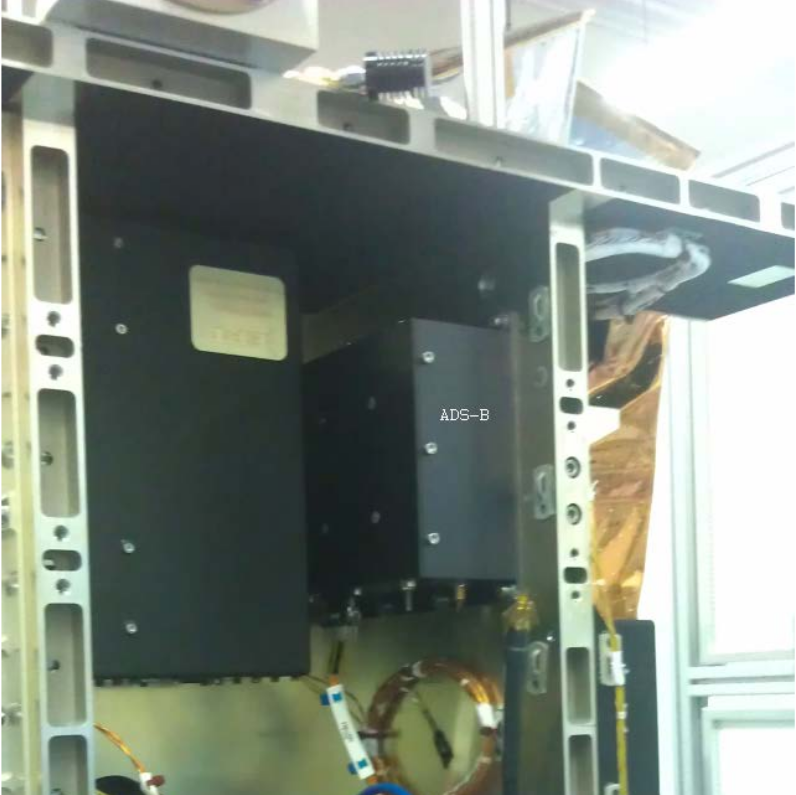
\includegraphics[width=1\linewidth]{pic/aos_ads-b_payload_1.png}
\end{minipage}}
\subfigure[卫星原型]{
\begin{minipage}[b]{0.3\linewidth}
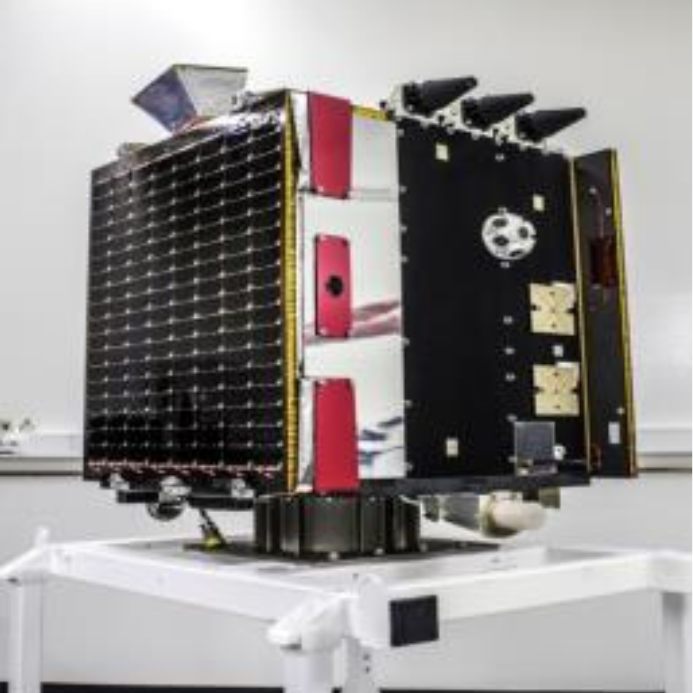
\includegraphics[width=1\linewidth]{pic/aos_ads-b_payload_3.png}
\end{minipage}}
\caption{Proba-V 卫星上搭载的 ADS-B 载荷}
\label{fig:aos_ads-b_payload}
\end{figure}

\begin{figure}[htbp]
\centering
\begin{minipage}[t]{0.48\textwidth}
\centering
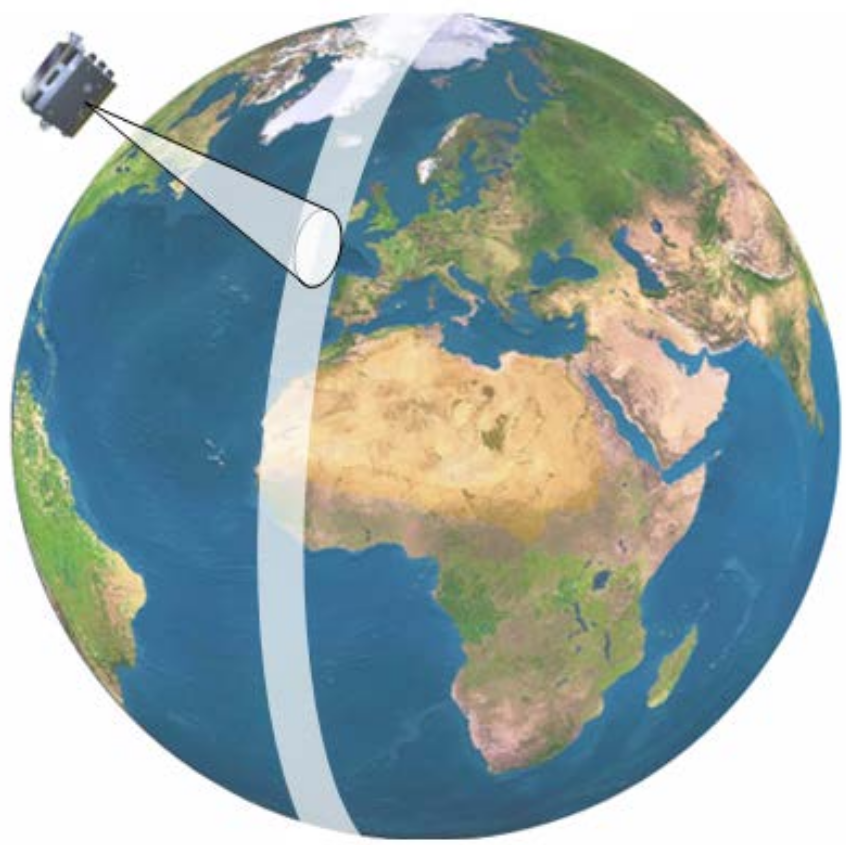
\includegraphics[width=6cm]{pic/aos_in_orbit.png}
\caption{技术验证阶段的单颗卫星}
\label{fig:aos_in_orbit}
\end{minipage}
\begin{minipage}[t]{0.48\textwidth}
\centering
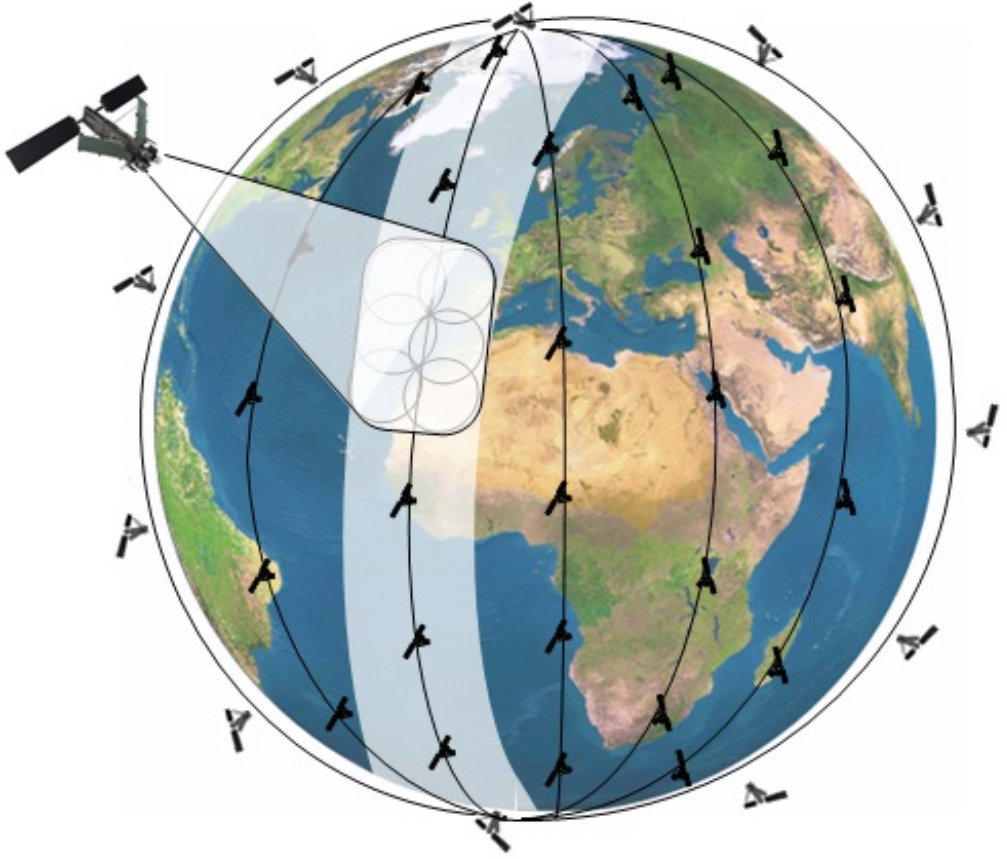
\includegraphics[width=7.2cm]{pic/aos_in_future.png}
\caption{未来全球卫星组网方案}
\label{fig:aos_in_future}
\end{minipage}
\end{figure}

\subsection{实验结果}

图\ref{fig:ADS-B_Auto6}展示了 2014 年 2 月 11 日在世界范围内记录的飞机航迹,每个红点代表卫星在其轨道上通过飞机时所看到的飞机航迹段。Proba-V 卫星的天线覆盖范围为纵向约 1200 公里,横向延伸至卫星飞行方向 500 公里,可逐条扫描全球空域。

\begin{figure}[htbp]
\centering
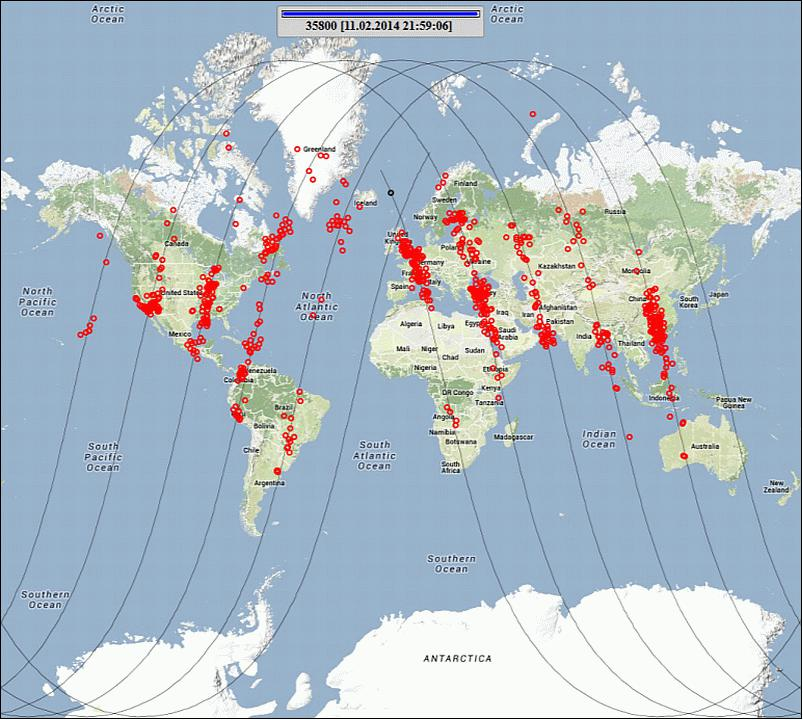
\includegraphics[width=10cm]{pic/ADS-B_Auto6.jpeg}
\caption{AOS 在世界范围内记录的飞机航迹(2014 年 2 月 11 日)}
\label{fig:ADS-B_Auto6}
\end{figure}

在空间接收 ADS-B 报文的最重要方面是卫星上 1090 MHz 扩展电文信号的接收条件。与基于地面的 ADS-B 监视相比,陆基 ADS-B 最大接收范围可达 300 公里,而在 820 公里高度轨道运行的 LEO 卫星与飞机之间的信号路径要长得多,这导致 ADS-B 的信号电平较低。接收器必须通过相关处理几乎在噪声水平上检测 S 模式信号。

实验得到了卫星天线覆盖区中不同区域接收到的 ADS-B 报文数量分布的直方图,如图\ref{fig:ADS-B_Auto5}所示,该图显示了 2014 年 5 月收到的所有位置消息的直方图。值得注意的是两个峰值,一个在卫星运动方向前方,峰值较低,另一个在卫星运动方向后方,峰值较高。这个谱的分布是不对称的,这由许多原因引起,比如卫星上的贴片天线的安装位置不对称、安装在卫星下侧的其他设备和在下表面的前边缘上突出的太阳能电池板。

\begin{figure}[htbp]
\centering
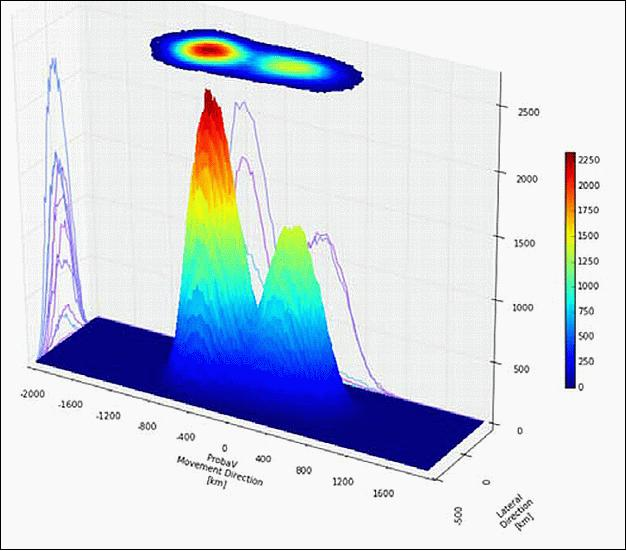
\includegraphics[width=10cm]{pic/ADS-B_Auto5.jpeg}
\caption{所有接收到的位置信息在天线覆盖区中的分布直方图}
\label{fig:ADS-B_Auto5}
\end{figure}

直方图的峰值可以通过卫星的接收天线和飞机的发射天线的天线辐射图来解释。图\ref{fig:ADS-B_Auto4}显示了安装在 Proba-V 卫星最低点面板上的 ADS-B 贴片天线的实测辐射图。合成的天线辐射图在卫星移动方向整体呈椭圆形状,最大灵敏度略低于卫星下方的最低点方向。

飞机装有两个 ATC 天线,一个在机身顶部,一个在机身底部,它们交替发射。由于几何因素限制,卫星将接收来自顶部天线的信号。顶部天线典型的垂直天线辐射模式如图\ref{fig:antenna_of_plane}所示。

\begin{figure}[htbp]
\centering
\begin{minipage}[t]{0.48\textwidth}
\centering
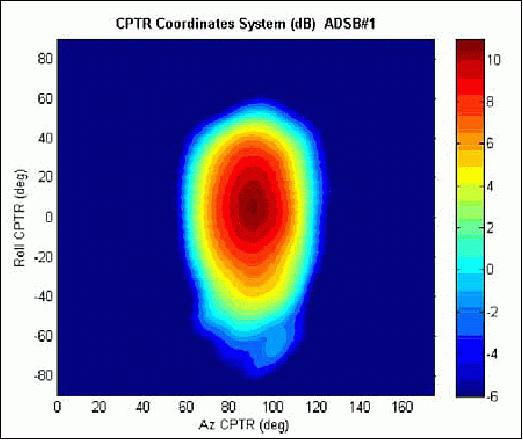
\includegraphics[width=7.5cm]{pic/ADS-B_Auto4.jpeg}
\caption{Proba-V 卫星天线辐射图}
\label{fig:ADS-B_Auto4}
\end{minipage}
\begin{minipage}[t]{0.48\textwidth}
\centering
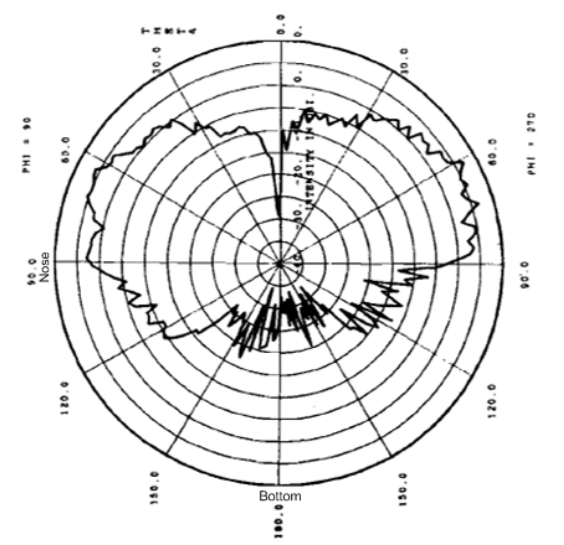
\includegraphics[width=6.5cm]{pic/antenna_of_plane.png}
\caption{顶部安装的 L 波段天线的垂直天线辐射图}
\label{fig:antenna_of_plane}
\end{minipage}
\end{figure}

\subsection{项目意义}

这次星载 ADS-B 接收验证实验的创举,将带来更多的在轨验证任务。ESA 与 Thales 德国签订合同,开发下一代 ADS-B 系统,该系统正在按计划进行,同时带来了卢森堡航天界(如 LuxSpace)的大力参与,将 TRITON 微小卫星平台作为以后的实验平台\upcite{h2}。

Proba-V 卫星实验项目取得了多个成果,主要包括:

\begin{itemize}
    \item 接收器的 FPGA 固件中包含一项特殊功能:允许上载新配置文件并通过远程访问激活这些配置。到目前为止,在任务运行期间,已成功测试了几次;

    \item 开发了改进的 S 模式相关机制,这得益于脉冲序列从第一个到第五个前导脉冲的相位相干性。在实验室测试中,可以显示报文检测率显著增加;

    \item 通过为 DF17 中的 112 个 S 模式数据位生成并保存“低置信度位”,增加了一次可以提高后处理报文解调成功率的机会;

    \item 卫星上的 ADS-B 接收器是同类中的第一个实验,接收从飞机发射的 1090ES ADS-B 电文信号。因此无法根据以往经验或任何结果进行系统设计。
\end{itemize}

Proba-V 卫星在实验中也遇到了一些困难,主要包括:

\begin{itemize}
    \item 由于卫星在大约 820 公里的高度,而飞机在 0 到 12 公里的高度,距离会导致接收的信号幅度过低从而导致信号丢失;

    \item 由于卫星天线垂直辐射图和飞机天线垂直辐射图的形状不同,会导致信号损失;

    \item 当到达卫星 ADS-B 天线的消息在时间上重叠(交织)时,ADS-B 接收机无法对其进行解码;

    \item 卫星的速度约为 27000 公里/小时,这导致每个检测到的飞机的观察时间有限,最多约 3 分钟。
\end{itemize}

这些困难提供了巨大的借鉴意义,为星基 ADS-B 技术发展中探明了一些需要克服的难点问题。

\section{Aireon 星基 ADS-B 系统}

\subsection{系统概述}

Aireon 星基 ADS-B 系统是搭载于第二代铱星(Iridium Next)卫星上的,作为第二代铱星星座系统提供服务的一部分。

\subsubsection{利益攸关方}

Aireon 的星基 ADS-B 系统的利益攸关方如表\ref{tab:stakeholders_of_Aireon_ads-b}所示。

\renewcommand\arraystretch{1.5}
\begin{table}[htbp]
\centering
\caption{Aireon 星基 ADS-B 系统的利益攸关方}
\label{tab:stakeholders_of_Aireon_ads-b}
\begin{tabular}[b]{|p{6cm}<{\raggedleft}|p{8cm}<{\raggedright}|}
\hline
\textbf{Iridium} & 卫星星座的拥有者和运营方 \\
\hline
\textbf{Aireon} & Iridium 和 NAV CANADA 的合资企业,旨在建立 ADS-B 服务 \\
\hline
\textbf{TAS(Thales Alenia Space)}& 卫星建造商,与 Iridium 签订合同 \\
\hline
\textbf{Harris Corporation} & ADS-B 有效载荷的建造商,与 Aireon 签订合同 \\
\hline
\textbf{ITT-Exeils} & 系统工程支持提供商,与 Aireon 签订合同,是处理和分销子系统的建造商 \\
\hline
\textbf{NAV CANADA} & Aireon 的投资方,为 ADS-B 服务启动客户 \\
\hline
\end{tabular}
\end{table}

\subsubsection{背景}

2012 年 11 月,铱星通信公司与 NAV CANADA 合资建立了 Aireon LLC 公司,这家合资企业将允许全球各地的空中交通管理机构持续跟踪世界各地的飞机。有史以来第一次,全球各地的 ANSP(空中导航服务提供商)将能够从极地到极地的追踪飞机,包括海洋空域和偏远地区。这将为航空业带来显著效益,包括大幅节省燃料,减少温室气体排放,提高安全性和效率等。该合资企业将在 FAA、行业和世界主要 ANSP 之间的 PPP(公私合作伙伴关系)下运营。

NAV CANADA 是一家加拿大的 ANSP,是 Aireon 的第一个客户,因为它管理着第二大空中导航服务并且是跨洋服务最大的提供商。

2014 年,Aireon LLC 成为 NAV CANADA、IAA(Irish Avation Authority)、ENAV(Ente Nazionale per l'Assistenza al Volo, Italy)、NAVIAR (Navigation Via Air, Denmark) 和 Iridium 共同的合资企业,用于融资、开发、部署并使用星基 ADS-B 接收器运行全球解决方案,以便在世界任何地方跟踪和监控飞机。\upcite{h2}

\subsubsection{铱星历史}

\begin{enumerate}
    \item[\textbf{初代铱星}]

    铱星卫星星座(Iridium satellite constellation)是在 20 世纪 90 年代初构想出来的,主要目的是提供全球卫星通讯服务。早期的计算表明需要 77 颗卫星,因此取名为铱星,这是由于这个卫星星座系统的结构类似于化学元素依(原子序数为 77,原子核周围有 77 个电子)。后来的事实证明,只需要 66 颗卫星即可完成对地球的全面覆盖。

    第一代铱星星座由 Iridium SSC(铱星通讯公司的前身) 开发,由摩托罗拉赞助。这些卫星于 1997-2002 年部署。第一代铱星卫星由美国、俄罗斯和中国的运载火箭发射,其中美国的 Delta II 火箭发射其中的 60 颗卫星;俄罗斯的 Proton-K/DM2 火箭发射其中的 21 颗卫星,1 枚 Rokot/Briz-KM 火箭发射其中的 2 颗;中国的“长征 2 号丙改进型”火箭发射其中的 12 颗卫星。

    第一代铱星全球覆盖于 2002 年完成,虽然系统满足其技术要求,但在市场上并不成功。传统地面移动通信几乎完全占领市场,铱星电话无法形成稳定的客户群,摩托罗拉公司未能获得足够的收入来偿还与建造星座相关的债务,而铱星公司则于 2000 年 3 月 17 日宣布破产,这是当时美国历史上最大的破产案。

    在最初的铱星公司宣布破产后,铱星星座系统仍然存在。铱星在2001年接受不足建设投资的 1\% (4800万美元)新注资后起死回生,美国军方是它主要客户,还被用于伊拉克战争,负责美军以及美军与盟军之间的协调行动。2010年,铱星通信与波音公司就卫星网络的维护,运行和支持达成了长期协议,波音运营星座,并为铱星的卫星控制系统(SCS)提供支持\upcite{h4}。

    尽管基于 LM-700A 型号的原始卫星预计设计寿命仅为 8 年,但 2002 - 2017 年没有发射新卫星来补充星座。

    \item[\textbf{第二代铱星}]

    2008 年 8 月,铱星选择了 Lockheed Martin 和 Thales Alenia Space 两家公司参与下一代卫星星座的采购竞标。2010 年 6 月,该合同的获胜者为 Thales Alenia Space。SpaceX 已经签约将会发射所有的 Iridium NEXT 卫星。Iridium NEXT 卫星如图\ref{fig:IMG_Iridium-Satellite_NEXT-Satellite-Vehicle}所示。

    \begin{figure}[htbp]
    \centering
    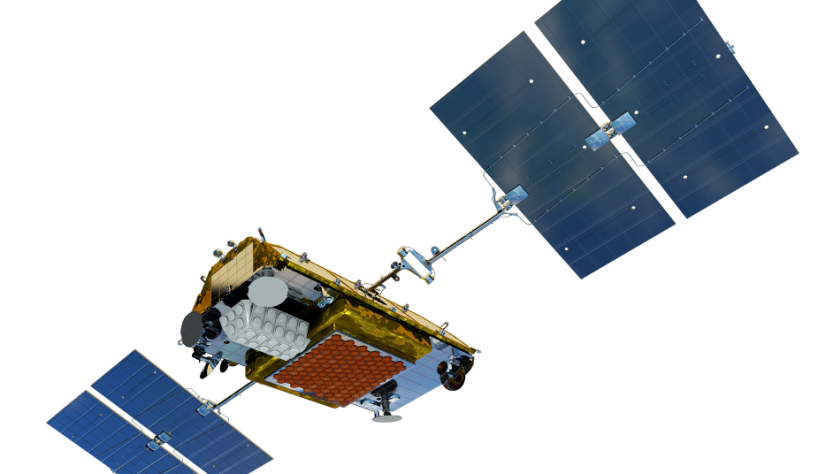
\includegraphics[width=13cm]{pic/IMG_Iridium-Satellite_NEXT-Satellite-Vehicle_HR_FEB16-clip-833x474.png}
    \caption{第二代铱星卫星}
    \label{fig:IMG_Iridium-Satellite_NEXT-Satellite-Vehicle}
    \end{figure}

    \renewcommand\arraystretch{1.5}
    \begin{table}[htbp]
    \centering
    \caption{第二代铱星卫星基本参数}
    \label{tab:iridium_next_paras}
    \begin{tabular}[b]{|p{4cm}<{\raggedleft}|p{8cm}<{\raggedright}|}
    \hline
    \textbf{帆板展开后翼展} & 9.4m \\
    \hline
    \textbf{卫星质量} & 约 860kg\\
    \hline
    \textbf{帆板收起时尺寸}& 3.1m x 2.4m x 1.5m \\
    \hline
    \textbf{轨道} & 圆极轨道(低地球轨道,LEO),海拔 780km,倾角 86.4$^\circ$,周期 101min(所有卫星总共分布于 6 个轨道上,每条轨道上包含 11 颗卫星)\\
    \hline
    \end{tabular}
    \end{table}

    2017 年 1 月,第二代铱星(Iridium NEXT)卫星开始部署到现有的星座中,Iridium SSC 的继承公司铱星通信公司(Iridium Communications)已经订购了由 Thales Alenia Space 和 Orbital ATK 共建造的共 81 颗新卫星,包括 66 颗在轨卫星,9 颗在轨备用卫星和 6 颗地面备用卫星。

    2017 年 1 月 14 日,第一批共 10 颗 Iridium NEXT 卫星发射成功,标志着该星座部署正式开始。最近的一次发射在 2019 年 1 月 11 日完成,SpaceX 的猎鹰 9 火箭将最后 10 颗卫星送入轨道,将 Iridium NEXT 星座数量增加到 75 颗(66 颗在轨卫星 + 9 颗在轨备用卫星),标志着 Iridium NEXT 星座部署正式完成。

    Iridium NEXT 卫星提供了 L 波段高达 128 kbit/s 的移动终端数据传输速度,高达 1.5 Mbit/s 的航海终端数据传输速度,用于固定/可移动终端的数据传输速度高达 8 Mbit/s。

    Iridium NEXT 为 Aireon 提供了二级载荷,是一个 ADS-B 接收器,并通过 FlightAware 软件由航空公司和空管使用,ADS-B 接收器原型如图\ref{fig:Appstar_with_Base}所示,接收器在卫星上的搭载位置如图\ref{fig:reconfigurable_multimission_payloads}所示。58 颗卫星上的三级载荷是加拿大 exactEarth 公司的海洋 AIS 船舶跟踪接收器。Iridium NEXT 还提供与太空中其他卫星的数据链接。\upcite{h3}

    \begin{figure}[htbp]
    \centering
    \begin{minipage}[t]{0.48\textwidth}
    \centering
    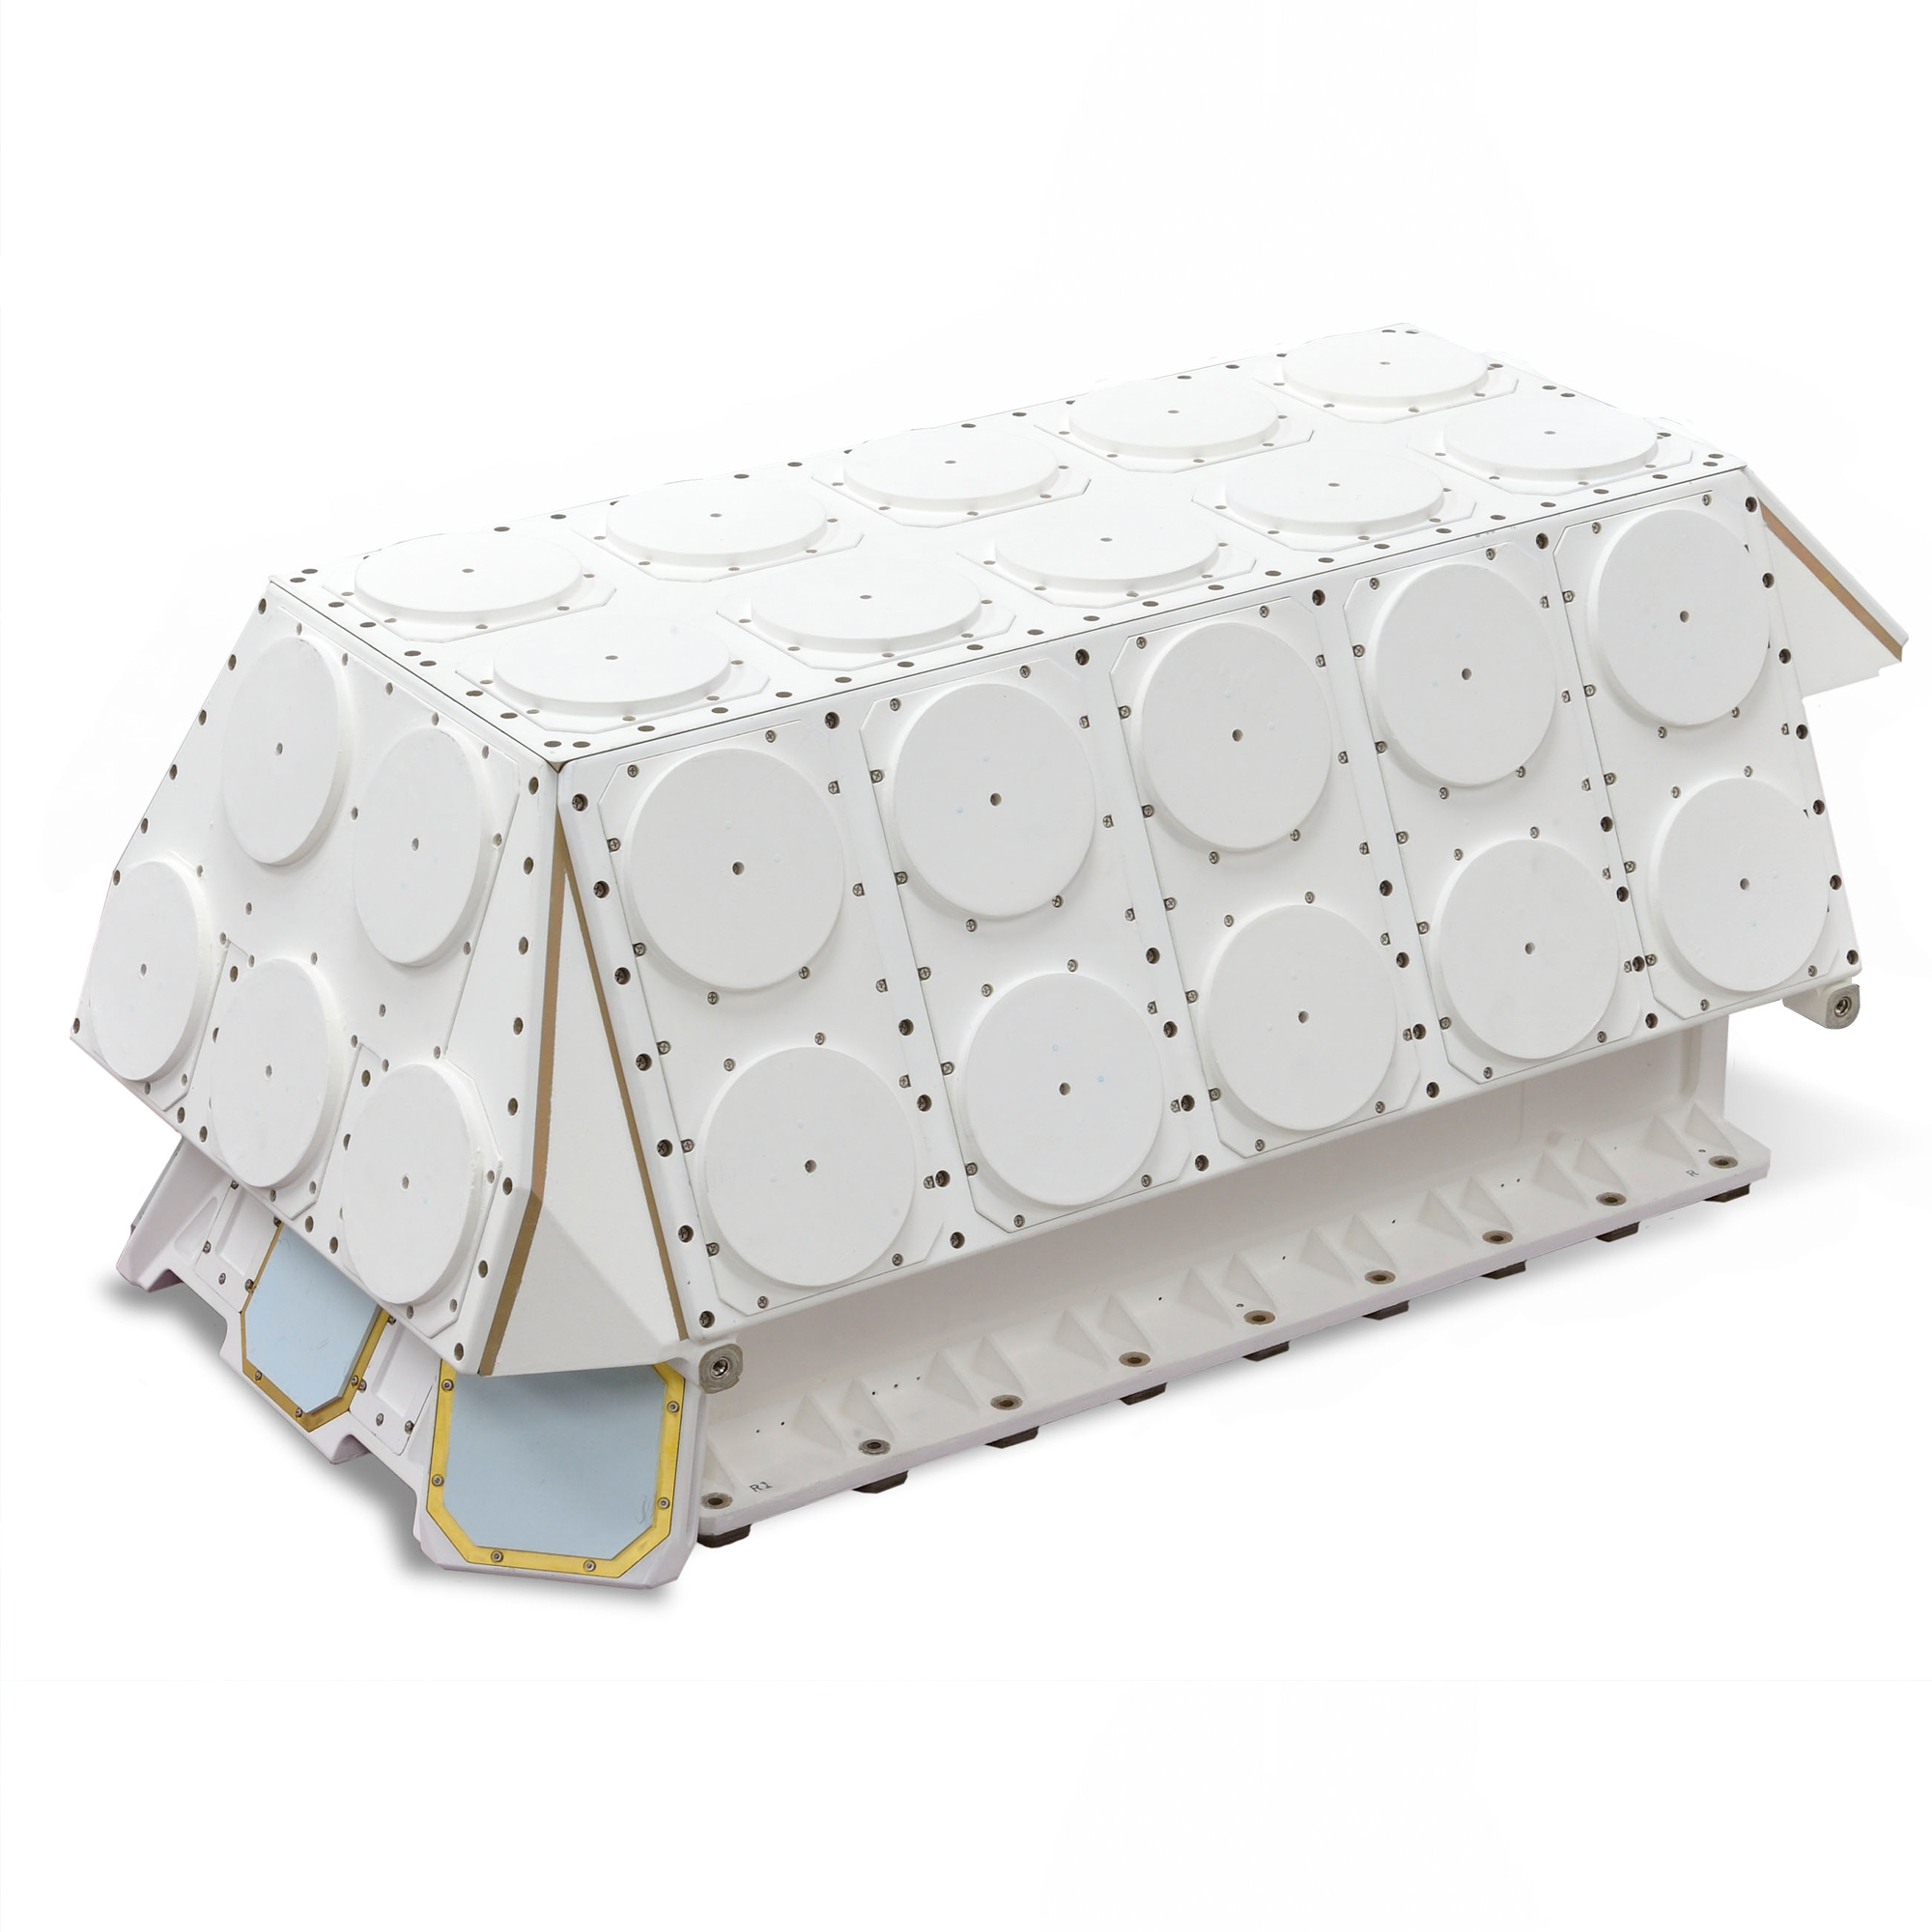
\includegraphics[width=6.5cm]{pic/Appstar_with_Base_2000x2000.jpg}
    \caption{Iridium NEXT 上的 ADS-B 接收器}
    \label{fig:Appstar_with_Base}
    \end{minipage}
    \begin{minipage}[t]{0.48\textwidth}
    \centering
    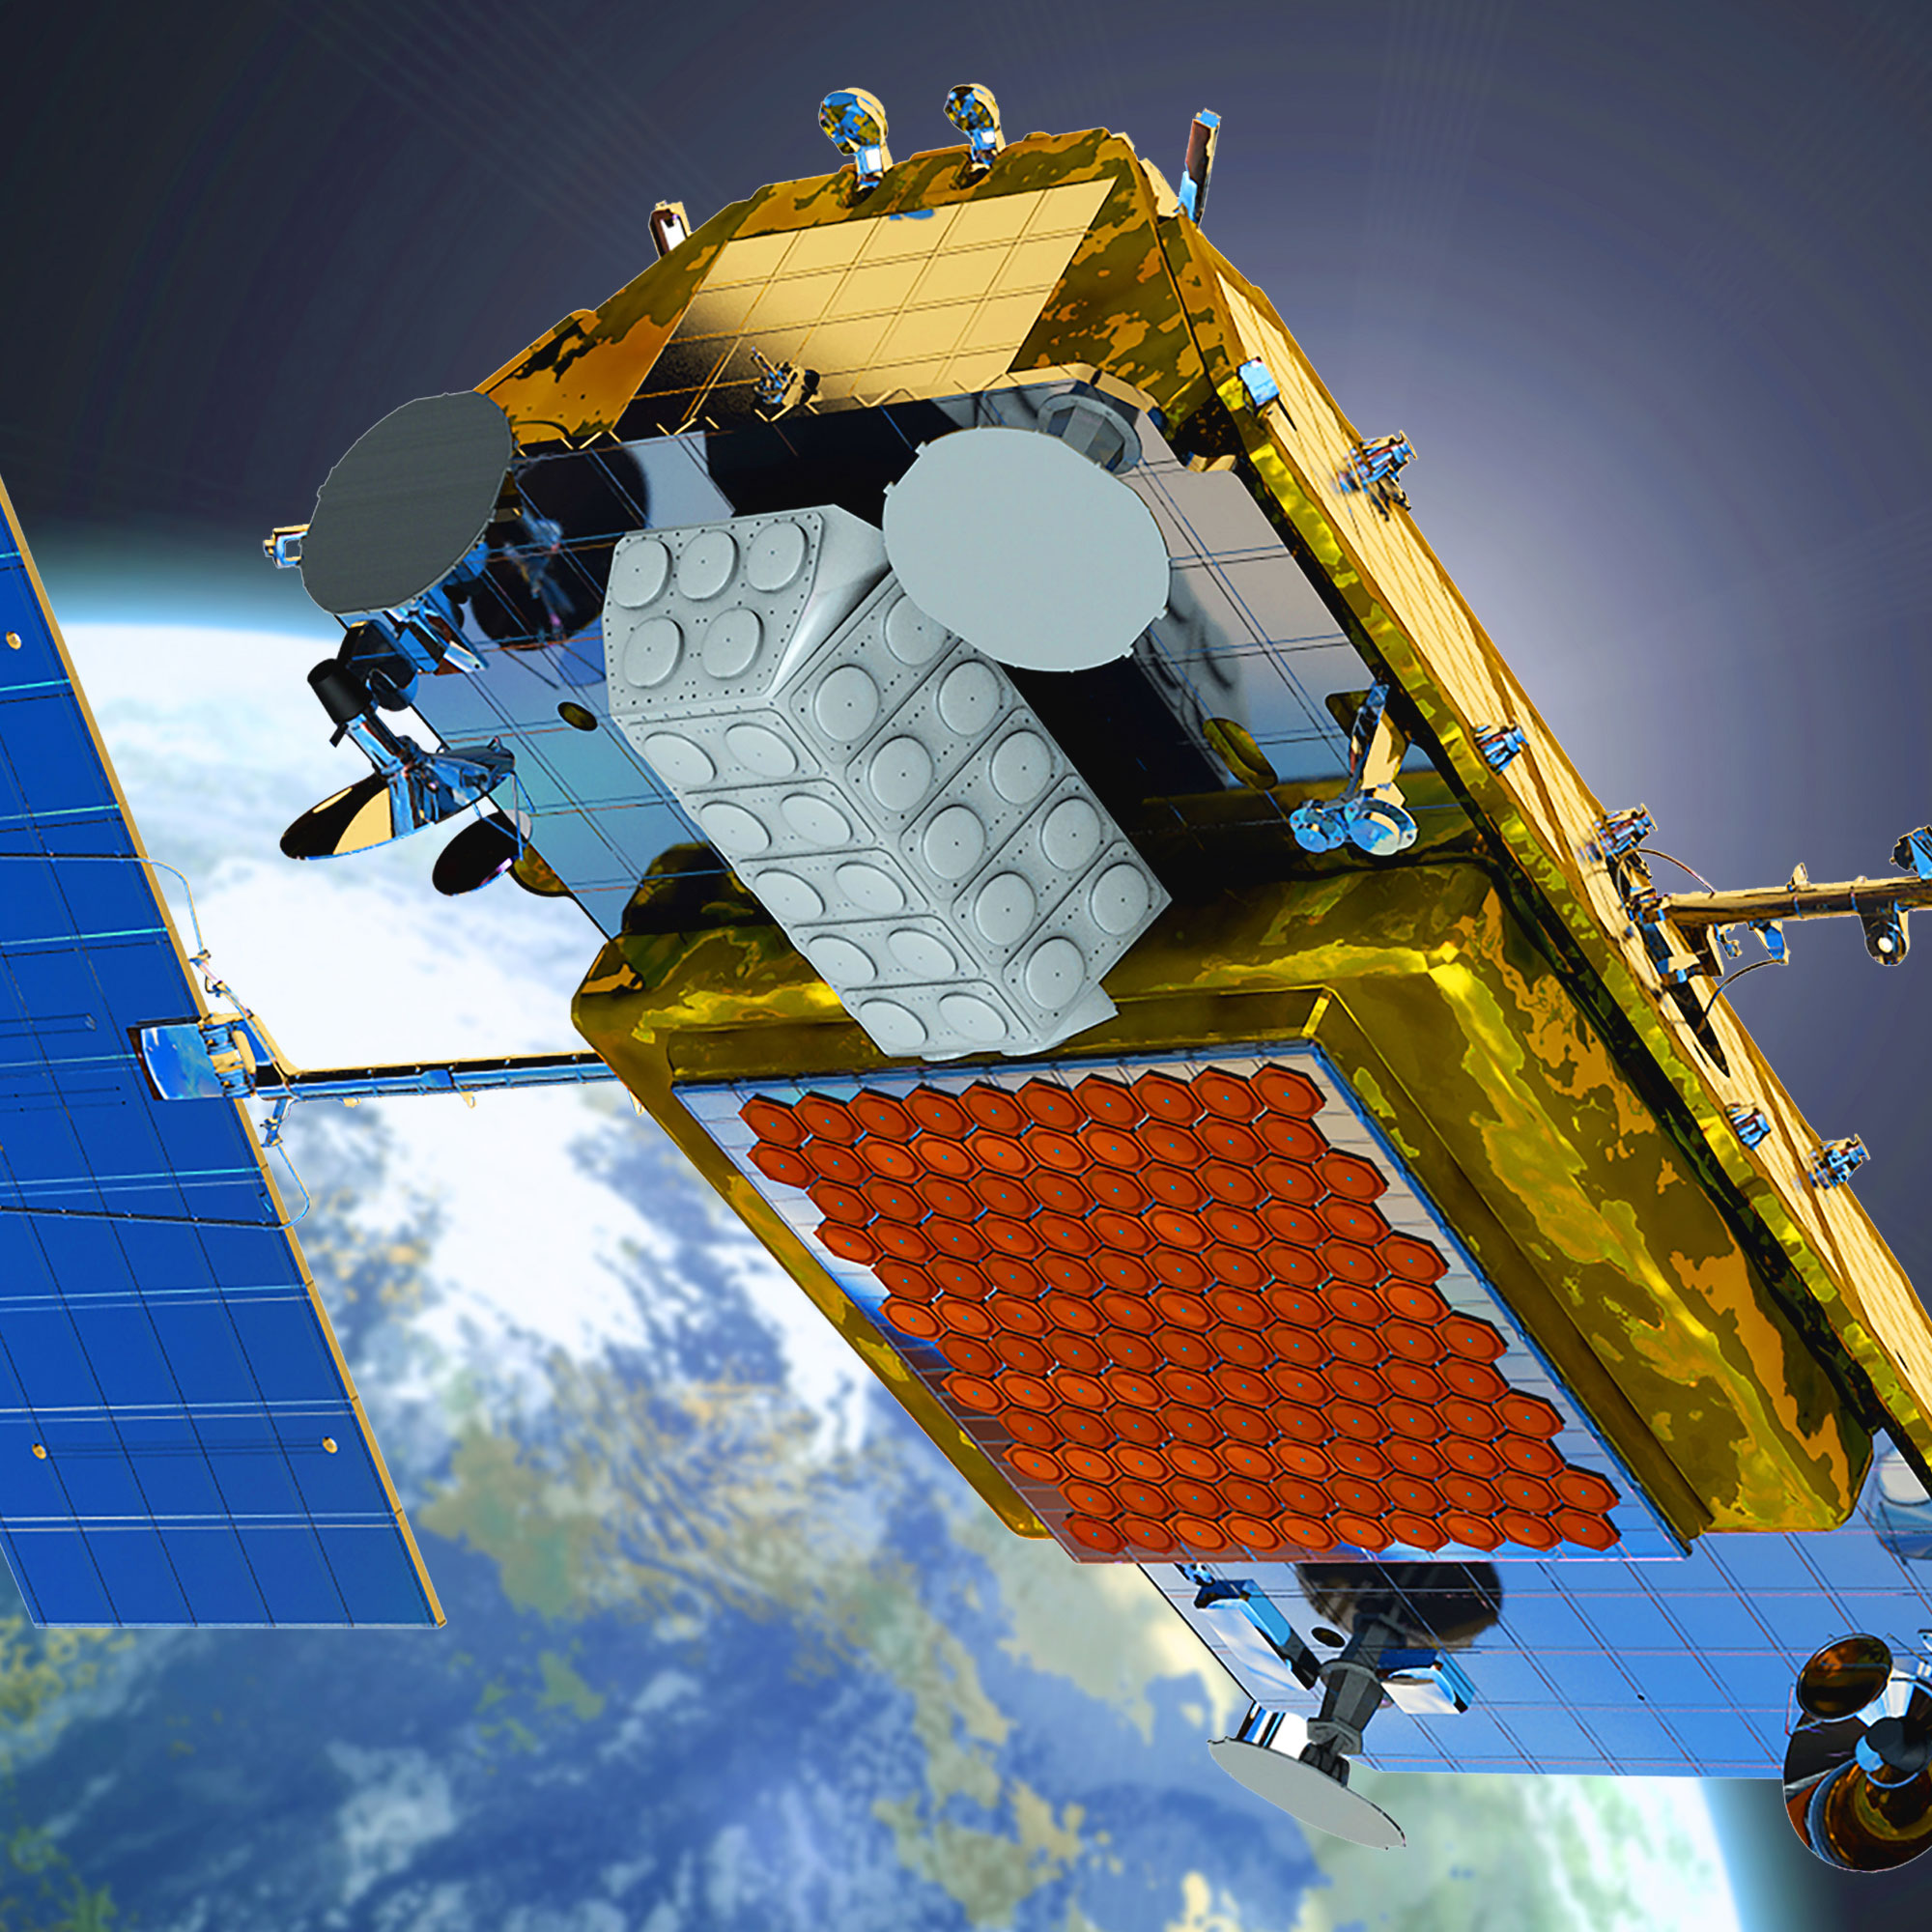
\includegraphics[width=6.5cm]{pic/reconfigurable_multimission_payloads_v2_web.jpg}
    \caption{ADS-B 接收器搭载方式}
    \label{fig:reconfigurable_multimission_payloads}
    \end{minipage}
    \end{figure}

\end{enumerate}

\subsection{体系结构}

Aireon 的星基 ADS-B 系统布局原理如图\ref{fig:Aireon_GlobalSpaceBasedADSB_Coverage_Diagram}所示。

\begin{figure}[htbp]
\centering
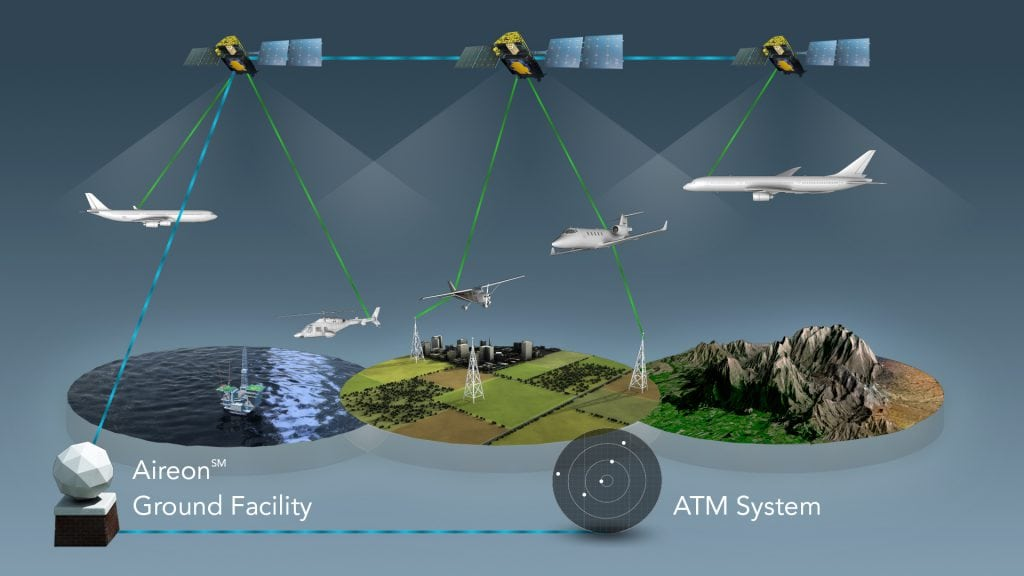
\includegraphics[width=14cm]{pic/Aireon_GlobalSpaceBasedADSB_Coverage_Diagram-1024x576.jpg}
\caption{Aireon 天基 ADS-B 系统布局原理}
\label{fig:Aireon_GlobalSpaceBasedADSB_Coverage_Diagram}
\end{figure}

如图\ref{fig:System-Diagram-1024x693}所示,从飞机上广播的 ADS-B 信息将由 Harris 建造的有效载荷(AHP)接收,AHP 将接收到的数据在卫星之间互传,然后下行传至 Aireon 的地面传送网络(TPN)和 Aireon 的处理和分配系统(APD)。在合作伙伴 Harris 的帮助下,APD 对数据进行解码和验证,并将数据传递给购买了 Aireon 服务的客户。

\begin{figure}[htbp]
\centering
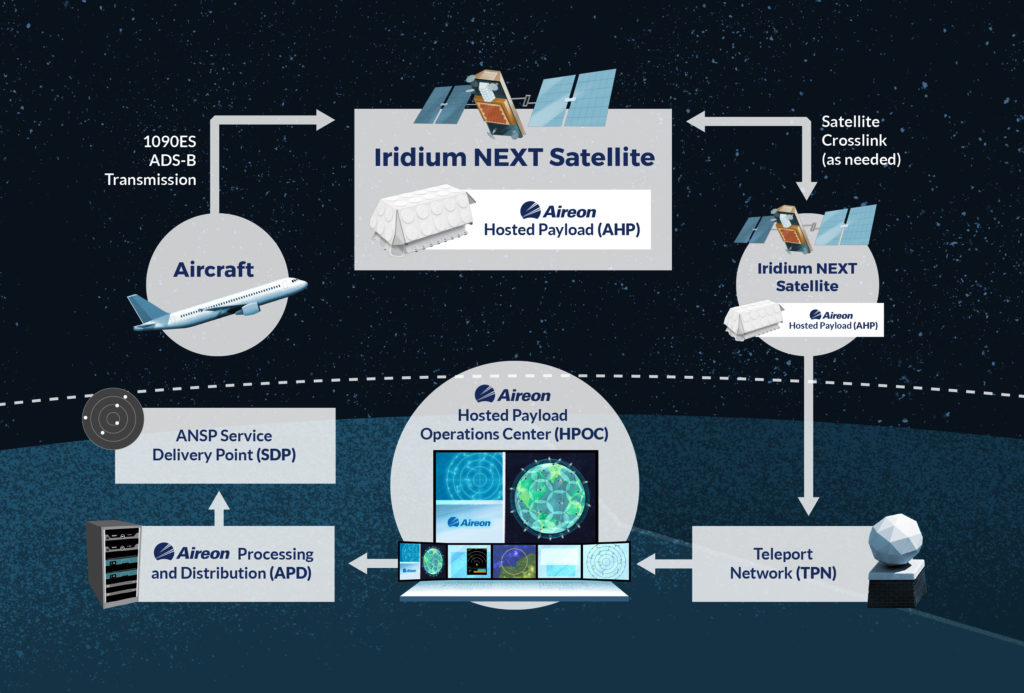
\includegraphics[width=13cm]{pic/System-Diagram-1024x693.jpg}
\caption{Aireon 天基 ADS-B 系统架构}
\label{fig:System-Diagram-1024x693}
\end{figure}

\subsection{系统性能}

Aireon 的星基 ADS-B 系统,目前只考虑了在卫星上安装 1090ES ADS-B 接收机,没有考虑安装 1090ES ADS-B 发射机。因此,该系统主要用于飞行监视和追踪,没有 TIS/FIS 上传能力\upcite{z1}。它的主要性能如表\ref{tab:aireon_ads-b_performance_para}所示。

\renewcommand\arraystretch{1.5}
\begin{table}[htbp]
\centering
\caption{Aireon 星基 ADS-B 系统的性能}
\label{tab:aireon_ads-b_performance_para}
\begin{tabular}[b]{|p{2.2cm}<{\raggedleft}|p{10.5cm}<{\raggedright}|}
\hline
\textbf{适用性} & 兼容所有符合 DO-260 标准的 1090ES ADS-B 设备 \\
\hline
\textbf{覆盖范围} & 可实现全球范围内不间断的覆盖 \\
\hline
\textbf{可用性} & 大于 99.9\% \\
\hline
\textbf{容量} & 每个点波束 1000 架飞机 \\
\hline
\textbf{时延} & ATC 检测追踪小于 1.5s \\
\hline
\textbf{更新速率} & 95\% 的响应速度小于 8s \\
\hline
\textbf{部署} & 已经部署完毕,2018 年 9 月提供全球的星基 ADS-B 服务 \\
\hline
\end{tabular}
\end{table}


\section{ALAS 系统}

\subsection{系统概述}

根据\url{www.ads-b.com}网站给出的说法,他们将天基 ADS-B 系统称为 ADS-B 链路增强系统(ADS-B Link Augmentation System),简称为“ALAS”。通过该系统,地球上任何地方的任意一架飞机可以被实时地安全追踪。

\subsection{体系结构}

\subsection{系统性能}

依托“全球星二代”系统的 ALAS 系统端到端(end-to-end)测试性能数据如表\ref{tab:alas-paras}所示。 \footnote{数据来源:\url{http://www.ads-b.com/space-based.htm}}

\renewcommand\arraystretch{1.5}
\begin{table}[htbp]
\centering
\caption{使用全球星卫星的 ALAS 系统端到端测试性能}
\label{tab:alas-paras}
\begin{tabular}[b]{|p{4cm}<{\raggedleft}|p{11cm}<{\raggedright}|}
\hline
\textbf{适用性
(Applicability)} &
ALAS 是一种简单、质量轻、低成本的外围设备,可与现有的任何 1090ES 或 UAT 电子设备配合使用,保证正常的空-地和地-空 ADS-B 传输不会中断。ALAS 还旨在与任何国家现有的 ADS-B 地面基础设施兼容\\
\hline
\textbf{覆盖范围(
Coverage Area)} &
到 2016 年,100\% 覆盖美国本土(CONUS)、GOMEX、加勒比海(Caribbean)、北大西洋(NAT)和北太平洋(NOPAC);到 2019 年,100\% 覆盖剩余地区\\
\hline
\textbf{可用性(
Availability)} & 到 2016 年,可用性为 99.99\%;到 2019 年,可用性为 99.999\% \\
\hline
\textbf{容量(
Capacity) }& 每架卫星可容纳大于 3000 架飞机(approx 1,800sm diameter)\\
\hline
\textbf{时延(
Latency)} &  从飞机到地面小于 200 毫秒;从端到端小于 300 毫秒 \\
\hline
\textbf{更新率(
Update Rate)} & 1 秒 \\
\hline
\textbf{完整性(
Integrity)} & 10E-6 \\
\hline
\textbf{精度(
Accuracy)} &
UTC 时制下,在 98\% 的时间里,相同目标的 射频视距(RF line-of-sight)导出位置和天基 ALAS 导出位置之间的显示位置差异小于 50 英尺\\
\hline
\textbf{安全性(
Security)} & 独一无二的安全。ALAS 与每架飞机建立了独特的双向连接,可以抵抗入侵、干扰或欺骗,是唯一的可以轻松加密的 ADS-B 形式。简单的防篡改设计还可以包括一个自供电备用系统,该系统将在未经授权而关闭飞机的主 ADS-B 转发器的情况下继续广播飞机的位置 \\
\hline
\textbf{可扩展性(
Scalability)}  & 高。系统架构的成本相对较低且简单,通过增加更多卫星和/或地面站,可以提高覆盖范围,可用性和容量 \\
\hline
\textbf{部署(
Deployment)} & 马上准备好。该技术已经过超过 100 小时的飞行测试。Globalstar 在过去两年中发射了 24 颗新的第二代 ALAS 卫星。Essential Services could be deployed as early as 3Q2016 and Critical Services NLT 2019\\
\hline
\textbf{成本(
Cost)} & 低。由于 ALAS 不需要新的卫星或太空中的其他技术,因此 ANSP 的买入和重复成本很小。它还可以与现有的 ADS-B 地面基础设施轻松连接。The price point for Part 121 avionics is less than \$40k and installation should be in the 20-25 MH range for most commercial aircraft. \\
\hline
\end{tabular}

\end{table}